\chapter{Conclusions}
\label{cha:conclusions}

\begin{comment}
Chapter 7: Conclusions
This can be a short chapter summarizing what you have achieved and what you have learned from the achievement. It is different from the abstract. The main results of your work should be highlighted with a critical appraisal of them indicating the extent to which the objectives outlined in Chapter 1 have been met. Exaggerated claims are counterproductive here. Recommendations for further activity are often included in this chapter.
\end{comment}

The project set out to build an application that made personal finances easier to manage through the automation of the common steps that people go through when making a budget.

Existing finance applications were researched, highlighting the advantages and disadvantages of each, as well as identifying the features that users found useful, through use of reviews.
%
A key piece of the functionality, the prediction engine, was discussed, investigating a combination of existing techniques used to forecast financial spending, including MCMs and Weighted Arithmetic Means. 
%
The ethical implications of storing high risk personally identifiable information was assessed and considered with reference to application security and strong security practice.
%
This research was then used decide on the functionality of the application, the design and implementation of the prediction engine and used to ensure high security standards were met throughout the application.

Specific design and implementation challenges were discussed, highlighting the key background and technical knowledge that was gained in order to overcome the challenges faced.

The aim of the project was to build an application that implemented an intuitive way to view and manage personal finances, accurately predict a users future \glspl{transaction} based on their history, as well as upholding the high security expectations of such a service.
%
The final application was reviewed following the usage pattern of the average user, to outline the key features implemented and to give an idea of how it works.

The evaluation of the application indicates that these three objectives have been met. Preliminary research demonstrates that users enjoyed using the application and indicates the majority of participants would use it in the future if implemented as a full product. Testing with participant data shows that the average absolute error of the prediction engine was $PERCENTAGE\%$ for users with over three months historical information. Preliminary penetration testing, using both white-box and black-box testing indicated that the security protections put in place are effective.  However, the evaluation of the project was limited, due to the size of the user base, discussed further in \autoref{sec:limitations}. \todo{Complete this}

%\subsection{Does it do what it's supposed to?}
%\plan{Does it make accurate predictions (summarise the evaluation section)}
%\section{Reflection}
%\subsection{Challenges}

% unit tests
% handling external inconsistencies

%\subsection{Key Lessons}
%\plan{How to do prediction, password entropy, other stuff}

\section{Limitations} \label{sec:limitations}
The main limitation of the project was the scope of the test participants. A total of 20 testers signed up to participate in the project during it's development, uploading at least one month of transaction data. However, only 7 of these individuals uploaded more than 3 months of transaction history, which was the threshold for using training and testing to select a best fit weighting model. In addition the majority of the participants were peers of the author, which meant that the majority of evaluation and testing was performed using students.

More extensive testing using a broader spectrum of testers, who may require a variety of different features, or use the system in a different way, may provide a greater level of evaluation for the system.

A key difficulty when seeking participants were their concerns regarding data security and trusting the researchers with their personal information. It it hoped that by publishing the level of concern and detail that has gone into the design of the security of the application, including encryption of their personally identifiable information, that the effects of this concern can be limited.

If the project were to continue, a more open approach for recruiting participants could be taken, such as seeking alpha testers and feedback in online forums and news groups. This should lead to both larger numbers of participants and a wider variety in the users background to give a fairer picture of potential users. Due to the variety of formatting already seen in participant data, it may be appropriate to limit the participants to the UK. A continued concern would be the security of the application when opening it up to users on the Internet, therefore this would need to be addressed.

During the testing and evaluation there were many features suggested by users to improve the application to their individual preferences. Due to time restraints the majority of these were not implemented and it was decided it was more imperative to focus on the most important and most frequently requested features first. Further development could include the additional requested features to suit a greater variety of users.

Although the key functionality of the application was unit tested, tests of the business logic in the prediction engine and on key objects was limited. This limitation was due to the heavy reliance on data, and because the engine performs differently depending on the users history. To test this functionality in the future data with pre-calculated attributes would be need to be prepared and a separate database access for storing this testing data would need to be implemented.

\begin{comment}
SELECT user_id, MAX(  `dateposted` ) , MIN(  `dateposted` ) , DATEDIFF( MAX(  `dateposted` ) , MIN(  `dateposted` ) ) /30
FROM transaction
GROUP BY  `user_id` 
ORDER BY DATEDIFF( MAX(  `dateposted` ) , MIN(  `dateposted` ) ) ASC 
\end{comment}

\section{Further research}
Due to the nature and size of this project a wide variety of further research opportunities have been highlighted.

\subsection{Model Selection}
Currently, the application selects most appropriate weighting model to use for each users transactions by evaluating the pre-defined weighting models via their historical data, and selecting the one with the least total overall error.

\subsubsection{User Classification}
Given the wealth of information the application holds about the users, higher accuracy could potentially be achieved by classifying each user. The users could be classified in two different ways; using pre-defined groups, or using cluster analysis. 

To split the users into existing groups, the researchers could identify groups that they believed would exhibit similar spending patterns and characteristics. Users would identify which group they felt they fit into when signing up and this information would be used to define the characteritics of each group. Having chosen features that identify each group, the researchers could automatically classify the users without prompting them

Alternatively, the use of cluster analysis could be employed to determine the number of groups, as well as the members of groups. The objective of the clustering would be to group users that exhibited similar spending patterns together, so those that were most similar were together and more similar to those in other clusters. 

Having classified the users, the parameters in the prediction engine could be configured for each individual group rather than by user. In addition, it would allow similar users to be compared, which would allow statements such as `users similar to you spend, on average, 10\% more' to be made, and could perhaps be used to make savings suggestions to each user.  

Further research could investigate the reliability of the classification using different clustering algorithms and whether configuring the prediction engine per group leads to better results than per user.

\subsubsection{Model Selection}
\label{section:overfittingmodels}
Weighting models were currently selected by category. The users total transactions per month in a particular category were evaluated and the weighting model with the best fit is chosen for that category. Transactions were considered by category and by month. Data was split by category which was chosen as the number of transactions in each subcategory was low, and preliminary experimentation showed that  sub-categories would suit the same model as their category. Using months as the time period was selected as the majority of participant data contained regular monthly transactions such as household and mobile phone bills, and so considering the transactions at smaller time steps led to errors in the Markov Chain Model as the probability of a transaction not occurring increased.

However, different time periods and methods of splitting the data could be investigated. For example transactions at each individual transactor could be assigned their own model, or all spending below a certain value could use the same model. The time periods used to build the model, could be by month, weeks, days or perhaps even by day of the week. Use of a time period such as a day of the week would result in a more complected Markov Chain Model where samples such as `given that the last purchase was on a Wednesday' could be taken.

Further research could investigate the effects of using different grouping methods and time periods on the overall accuracy of the predictions.

\subsection{Alternative Forecasting Techniques}
\label{section:triplesmoothing}
The system currently uses techniques adapted from exponential smoothing to forecast and predict the value of a future transaction. Currently this is limited to a weighted arithmetic mean in the form shown in Fig. \ref{fig:weighted-mean}. Use of a mean to forecast the value of the next period performs poorly when there is a trend in the data \parencite{filliben2003nist}.

\begin{figure}
\centering
$\bar{x} = \frac{\sum^{n-1}_{t=0}{w(t) \times x_{t}}}{\sum_{t=0}^{n-1}{w(t)}}$
\caption{Weighted arithmetic mean}
\label{fig:weighted-mean}
\end{figure}

Second order or double exponential smoothing can be used to take into account trends and seasonal changes in data, such as the average value of an individuals weekly shop increasing over time, or the increase of purchases during Christmas. 
%
Double exponential smoothing involves two steps, calculating the weighted mean as before, and then adjusting that mean by the difference between the previous value and it's associated prediction, shown in Fig. \ref{fig:second-order-math}, the comparison between the weighted mean and second order forecasting transaction that is increasing in value by 10, for each time period is shown in Fig. \ref{fig:prediction-second}. 
%
Triple exponential smoothing extends the trend calculation to include a seasonal index. Assuming at least one complete seasons data is available the value of $x_t$ of scaled by this seasonal index, which is calculated using by taking the average value of this period historically and dividing it by the average value for the year that the period occurred or $S_{t} = \frac{x_t}{\bar{x}_p}$ and $\bar{x}_p = \frac{\sum_{i=1}^{p} x_i}{p}$ where $p$ is the number of periods in a year, and $x_i$ is the value of the period $i$ in the year considered. Fig. \ref{fig:prediction-third} shows the performance on some data that follows a similar trend to the previous year \parencite{kalekar2004holtwinters,dash2012movingaverages}.

Further research could investigate the effect of applying double order and triple exponential smoothing to forecast the values of transactions on the final prediction and how seasonal indexes could be calculated. Seasonal indexes, for example, could be calculated per transactor, category, user or globally across the application. The research would need access to historical transaction data for the users to be able to make these assessments.

\begin{figure}
\centering
\[\bar{x}_t = \alpha(t) \times \bar{x}_t + (1 - \alpha(t))(\bar{x}_{t-1} + b_t-1)\]
\[b_t = \alpha(t)(\bar{x}_t - \bar{x}_{t-1}) + (1 - \alpha(t))b_{t-1}\]

Where $\alpha(t) = \frac{w(t)}{\sum_{t=0}^{n-1}{w(t)}}$ representing the final weight\\
In general, the starting values are set as $\bar{x}_1 = x_1$ and $b_1 = x_2 - x_1$

\caption{Calculating the second order weighted arithmetic mean}
\label{fig:second-order-math}
\end{figure}

\begin{figure}
\centering
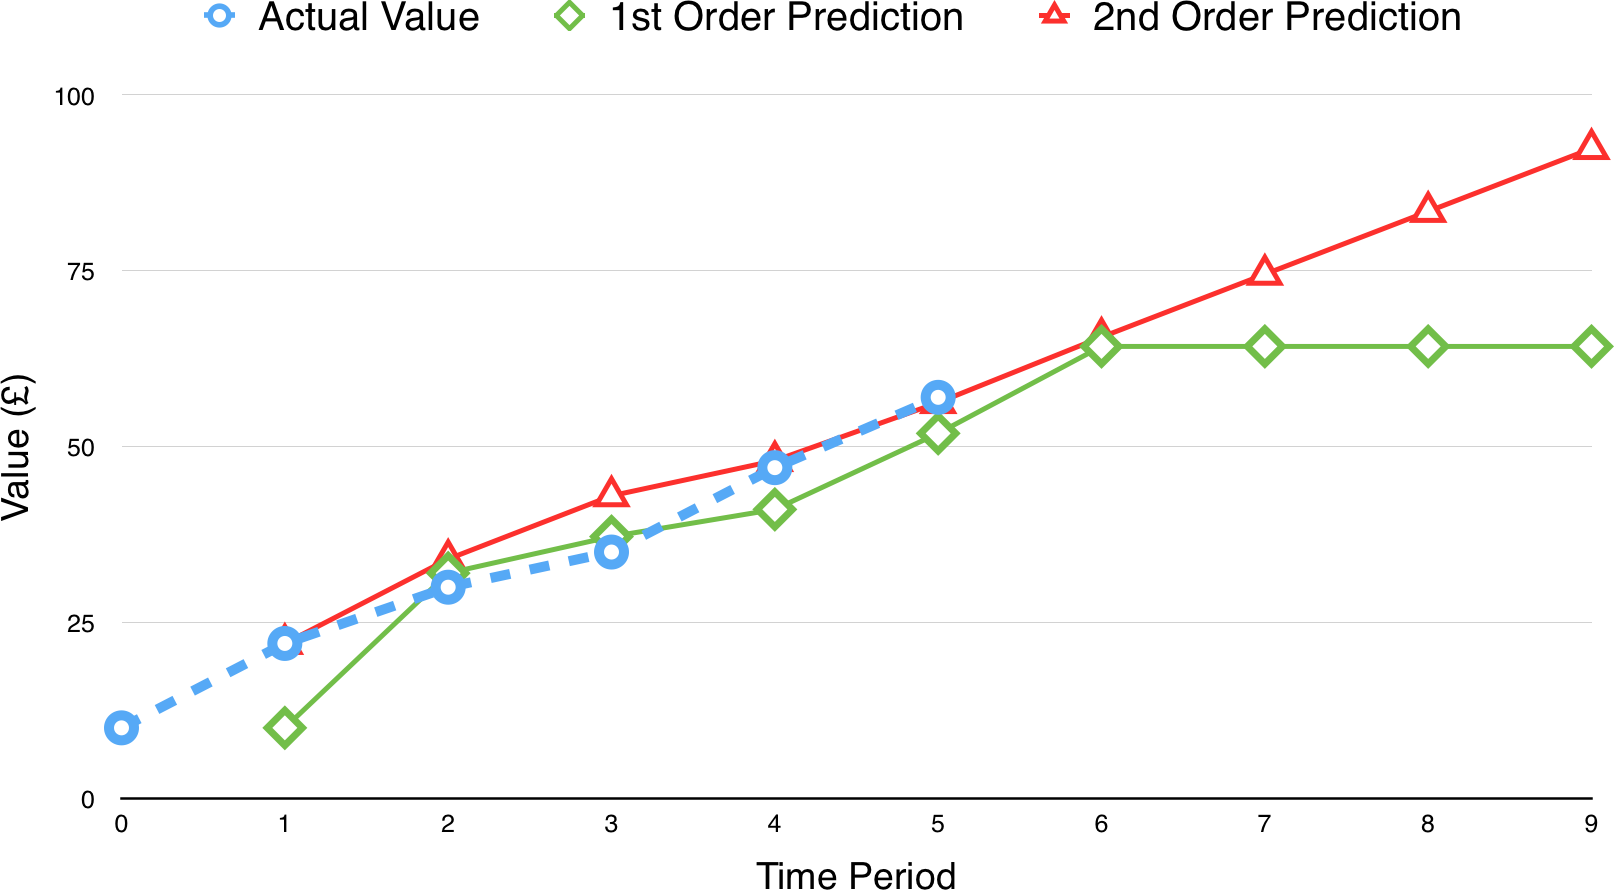
\includegraphics[width=0.75\textwidth]{conclusion/second-prediction}
\caption{Comparison of first and second order forecasting when predicting a trend}
\label{fig:prediction-second}
\end{figure}

\begin{figure}
\centering
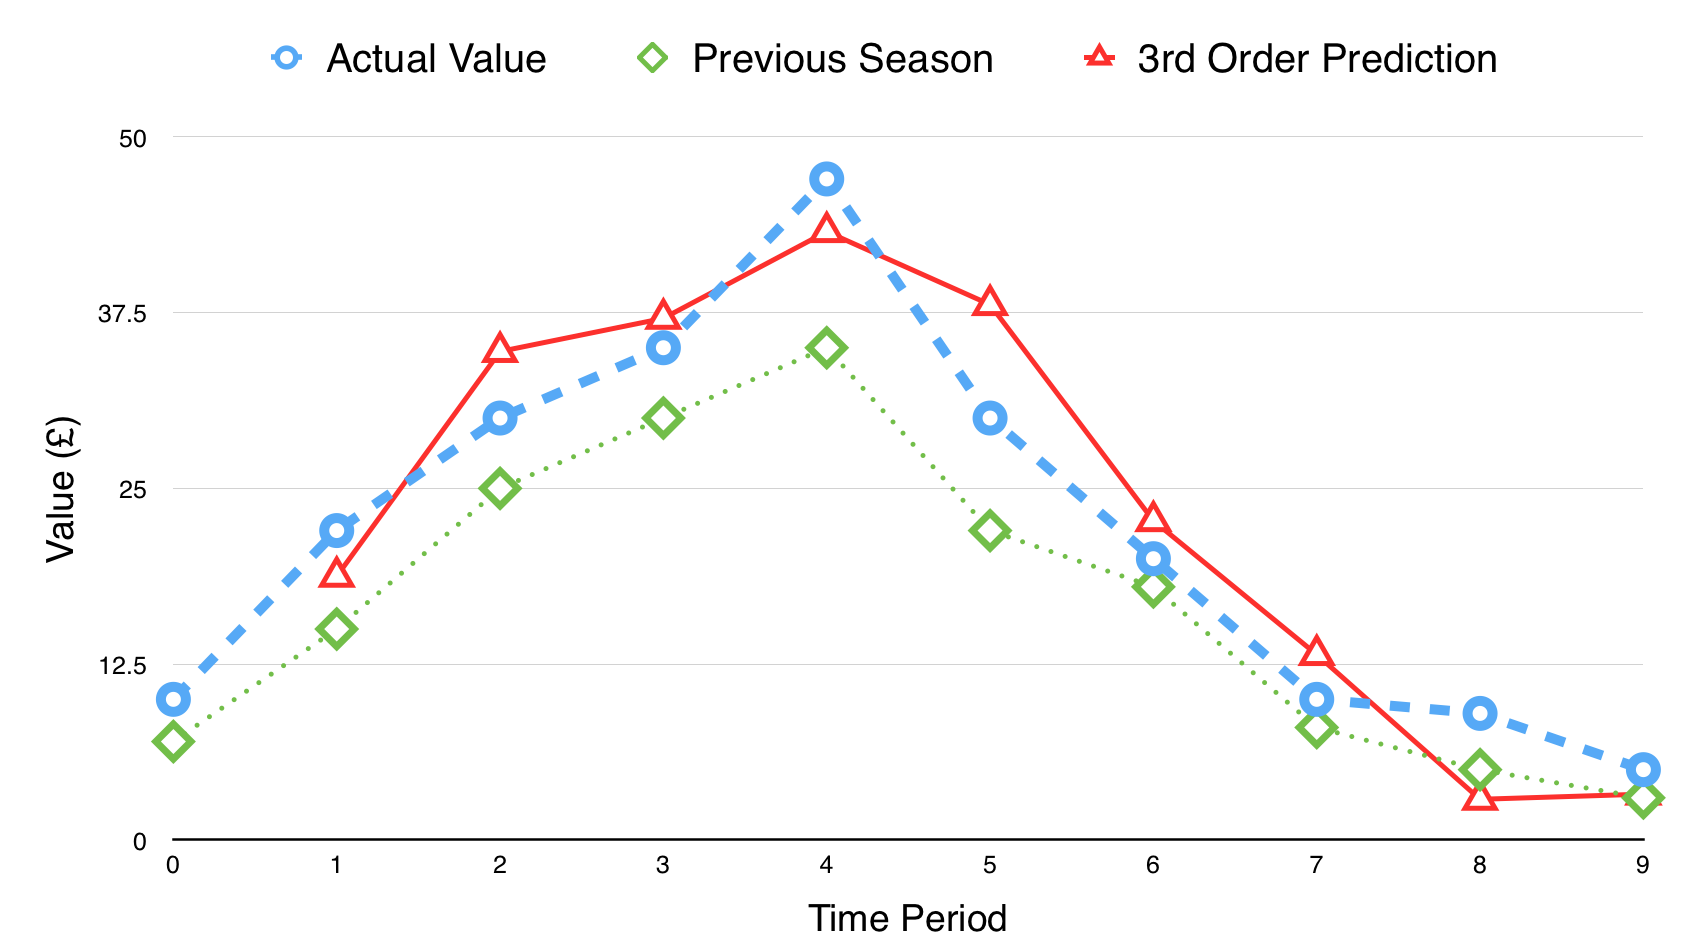
\includegraphics[width=0.75\textwidth]{conclusion/triple-prediction}
\caption{Using third order forecasting on data with a previous season}
\label{fig:prediction-third}
\end{figure}

\subsection{Learning the Scaling Parameters}
\label{section:learningscalingparameter}
It was mentioned in section \ref{sub:fivemodelsystem} that the speed of the decay in the weighting functions could adjusted by using a scaling constant. Instead of choosing the best weighting model from a pre-defined selection, the application could apply non-linear optimisation techniques to adjust the rate of the decay, and select a customised model for each user. 

Further research could investigate different implementations of these optimisation techniques, and how the use of custom models affects the prediction accuracy for each user.

